\documentclass[a4paper,10pt]{article}
\usepackage[brazilian]{babel}
\usepackage[left=2.5cm,right=2.5cm,top=3cm,bottom=2.5cm]{geometry}
\usepackage{mathtools}
\usepackage{amsthm}
\usepackage{amsmath}
%\usepackage{nccmath}
\usepackage{amssymb}
\usepackage{amsfonts}
\usepackage{physics}
%\usepackage{dsfont}
%\usepackage{mathrsfs}

\usepackage{titling}
\usepackage{indentfirst}

\usepackage{bm}
\usepackage[dvipsnames]{xcolor}
\usepackage{cancel}

\usepackage{xurl}
\usepackage[colorlinks=true]{hyperref}

\usepackage{float}
\usepackage{graphicx}
%\usepackage{tikz}
\usepackage{caption}
\usepackage{subcaption}

%%%%%%%%%%%%%%%%%%%%%%%%%%%%%%%%%%%%%%%%%%%%%%%%%%%

\newcommand{\eps}{\epsilon}
\newcommand{\vphi}{\varphi}
\newcommand{\cte}{\text{cte}}

\newcommand{\N}{\mathbb{N}}
\newcommand{\Z}{\mathbb{Z}}
\newcommand{\Q}{\mathbb{Q}}
\newcommand{\R}{\vb{R}}
\newcommand{\C}{\mathbb{C}}
\renewcommand{\S}{\hat{S}}
%\renewcommand{\H}{\s{H}}

\renewcommand{\a}{\vb{a}}
\newcommand{\nn}{\hat{n}}
\renewcommand{\d}{\dagger}
\newcommand{\up}{\uparrow}
\newcommand{\down}{\downarrow}

\newcommand{\0}{\vb{0}}
%\newcommand{\1}{\mathds{1}}
\newcommand{\E}{\vb{E}}
\newcommand{\B}{\vb{B}}
\renewcommand{\v}{\vb{v}}
\renewcommand{\r}{\vb{r}}
\renewcommand{\k}{\vb{k}}
\newcommand{\p}{\vb{p}}
\newcommand{\q}{\vb{q}}
\newcommand{\F}{\vb{F}}

\newcommand{\s}{\sigma}
%\newcommand{\prodint}[2]{\left\langle #1 , #2 \right\rangle}
\newcommand{\cc}[1]{\overline{#1}}
\newcommand{\Eval}[3]{\eval{\left( #1 \right)}_{#2}^{#3}}

\newcommand{\unit}[1]{\; \mathrm{#1}}

\newcommand{\n}{\medskip}
\newcommand{\e}{\quad \mathrm{e} \quad}
\newcommand{\ou}{\quad \mathrm{ou} \quad}
\newcommand{\virg}{\, , \;}
\newcommand{\ptodo}{\forall \,}
\renewcommand{\implies}{\; \Rightarrow \;}
%\newcommand{\eqname}[1]{\tag*{#1}} % Tag equation with name

\setlength{\droptitle}{-7em}

\theoremstyle{plain}
\newtheorem{theorem}{Teorema}[section]
%\newtheorem{defi}[theorem]{Definição}
\newtheorem{lemma}[theorem]{Lema}
%\newtheorem{corol}[theorem]{Corolário}
%\newtheorem{prop}[theorem]{Proposição}
%\newtheorem{example}{Exemplo}
%
%\newtheorem{inneraxiom}{Axioma}
%\newenvironment{axioma}[1]
%  {\renewcommand\theinneraxiom{#1}\inneraxiom}
%  {\endinneraxiom}
%
%\newtheorem{innerpostulado}{Postulado}
%\newenvironment{postulado}[1]
%  {\renewcommand\theinnerpostulado{#1}\innerpostulado}
%  {\endinnerpostulado}
%
%\newtheorem{innerexercise}{Exercício}
%\newenvironment{exercise}[1]
%  {\renewcommand\theinnerexercise{#1}\innerexercise}
%  {\endinnerexercise}
%
%\newtheorem{innerthm}{Teorema}
%\newenvironment{teorema}[1]
%  {\renewcommand\theinnerthm{#1}\innerthm}
%  {\endinnerthm}
%
\newtheorem{innerlema}{Lema}
\newenvironment{lema}[1]
  {\renewcommand\theinnerlema{#1}\innerlema}
  {\endinnerlema}
%
%\theoremstyle{remark}
%\newtheorem*{hint}{Dica}
%\newtheorem*{notation}{Notação}
%\newtheorem*{obs}{Observação}


\title{\Huge{\textbf{Introdução à supercondutividade não-convencional}}}
\author{Mateus Marques}

\begin{document}

\maketitle

\section{Introdução}

Dizemos que um supercondutor é não-convencional quando este não pode ser adequadamente descrito pela teoria BCS (Bardeen-Cooper-Schrieffer). A busca por um mecanismo que explique os diversos tipos de supercondutividade não-convencionais, apesar de antiga, ainda se configura como um dos temas de pesquisa mais importantes dentro da área da Física da Matéria Condensada Teórica. Em geral, espera-se que o entendimento da origem dos supercondutores de alta temperatura ajude na procura experimental por um material supercondutor à temperatura ambiente, o que possibilitaria poderosas aplicações tecnológicas, como a transmissão em larga escala de energia elétrica sem dissipação.

Os supercondutores de alta temperatura, especialmente os cupratos, são os mais acessíveis hoje em dia devido à $T_c$ ser maior que a temperatura de ebulição de $77 \unit{K}$ do nitrogênio líquido, que funciona como um refrigerante relativamente barato.

\begin{figure}[H]
\centering
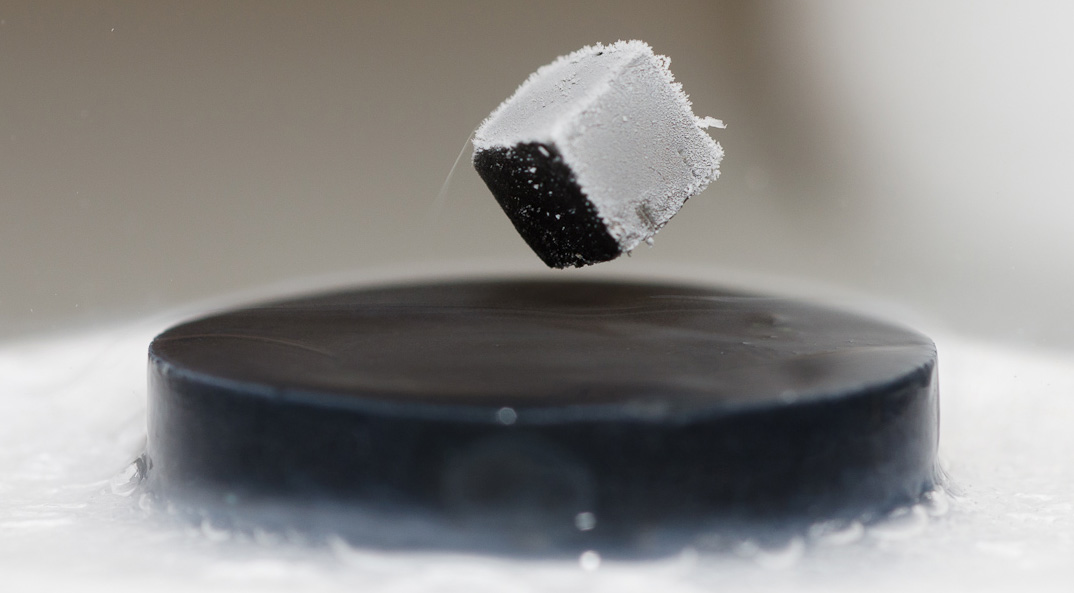
\includegraphics[width=0.7\textwidth]{fig/levitating.jpg}
\caption{Supercondutor de cuprato levitando sobre um ímã pelo efeito Meissner.}
\label{fig:levitating}
\end{figure}

%$$
%U_{\k\k'} =
%\begin{cases}
%\; -g, \text{ se } E_F \leq \eps(\k), \eps(\k') \leq E_F + \hbar \omega_D \\
%\; 0, \text{ caso contrário.}
%\end{cases}
%$$

Existe bastante diversidade dentre todos os supercondutores já conhecidos e é uma tarefa um pouco arriscada afirmar com exatidão as propriedades de um supercondutor específico, devido a isso se tratar de um tópico com uma quantidade enorme de pesquisa, discussão e controvérsia dentro da comunidade científica.

Seguindo \cite{wiki-history_superconductivity}, o primeiro supercondutor (convencional) descoberto foi o mercúrio (Hg) em 1911, tendo sido resfriado por hélio líquido e possuindo $T_c = 4.2 \unit{K}$. Nas décadas subsequentes outros supercondutores foram sendo descobertos, como o chumbo (Pb) e o nióbio (Nb). Na década de 1930 foi descoberto o efeito Meissner, em que supercondutores tendem a expulsar o campo magnético aplicado sobre eles. Esse efeito é uma manifestação muito atraente do estado supercondutor, pois permite que vejamos sua ação a olho nu em experimentos relativamente fáceis de fazer, como vemos na Figura \ref{fig:levitating} um supercondutor de cuprato, resfriado por nitrogênio líquido, levitando pelo efeito Meissner. Na década de 50 foi estabelecida a teoria BCS de supercondutividade, que conseguia explicar todos os supercondutores conhecidos até então. Seus autores John Bardeen, Leon N. Cooper e Robert Schrieffer compartilharam o prêmio Nobel pela teoria BCS em 1972.

Foi na década de 80 que iniciaram-se descobertas de supercondutores que não conseguiam ser descritos, por diferentes razões, pela teoria BCS. Seguindo a referência \cite{timm}, listaremos algumas em ordem cronológica:
\begin{itemize}
\item Em 1979 foi observado supercondutividade abaixo de $T_c \simeq 0.5 \unit{K}$ no Ce$_2$Cu$_2$Si$_2$, que não tem estado normal de metal, mas sim de um material heavy-fermion. Devido às grandes correlações dos elétrons de orbital $f$ do Ce, a massa efetiva do material excede muito a massa do elétron $m^* \gg m_e$.
\item Também em 1979 foi observado supercondutividade no sal orgânico (TMTSF)$_2$PF$_6$, com $T_c = 1.1 \unit{K}$. Desde então, foram descobertos outros supercondutores orgânicos com $T_c$ até da ordem de $18 \unit{K}$. Pensa-se que a simetria do estado supercondutor de vários desses materiais orgânicos é não-convencional (não s-wave).
\item O primeiro supercondutor de alta temperatura foi descoberto em 1986, pelos pesquisadores J. G. Bednorz e K. A. Müller da IBM, que identificaram supercondutividade no composto baseado em cuprato La$_{2-x}$Ba$_x$CuO$_4$, com $T_c \simeq 35 \unit{K}$. Eles obtiveram o prêmio Nobel no ano seguinte por tal descoberta. Nos anos subsequentes, vários outros supercondutores com estrutura cristalina contendo planos de CuO$_2$ (cupratos) foram descobertos. Os valores de $T_c$ dos cupratos são os maiores conhecidos até então à pressão ambiente.

\item Em 1994 descobriram supercondutividade no Sr$_2$RuO$_4$, que por muito tempo pensou que se tratava de uma simetria p-wave, assim como o estado superfluido do $^3$He. Porém experimentos recentes colocam isso em dúvida, mas sua supercondutividade é certamente não-convencional.

\item Em 2001 foi relatado supercondutividade no MgB$_2$ com $T_c = 39 \unit{K}$. Por ser uma temperatura crítica tão alta e o material possuir uma estrutura cristalina parecida com a dos cupratos, houve a expectativa de ser não-convencional. Porém, acredita-se que na verdade ele seja BCS.

\item Nos anos 2000 foi descoberta uma nova classe de supercondutores baseados em Fe$^{2+}$, batizados de pnictideos de ferro. Eles são curiosos pois, mesmo possuindo íons de ferro, vários materiais dessa classe possuem ordem antiferromagnética mas, diferentemente dos cupratos, eles são metálicos.
\end{itemize}

Na tabela \ref{tab:superconductors} abaixo listo exemplos de alguns supercondutores selecionados.

\begin{table}[H]
\begin{center}
\begin{tabular}{ |p{3cm}||p{3cm}|p{3cm}|p{3cm}|  }
\hline
Supercondutor & Simetria & $T_c \simeq$ & Categoria \\
\hline
Hg                   & s-wave    & $4.2   \, \text{K}$      & BCS \\
MgB$_2$              & s-wave    & $39    \, \text{K}$      & BCS \\
$^3$He               & p-wave    & $2.5   \, \text{mK}$     & Superfluido \\
Sr$_2$RuO$_4$        & $-$       & $0.93  \, \text{K}$      & $-$ \\
YBCO                 & d-wave    & $93  \, \text{K}$        & Cuprato \\
BSCCO-2223           & d-wave    & $108   \, \text{K}$      & Cuprato \\
UPt$_3$              & f-wave?   & $0.51  \, \text{K}$      & Heavy-Fermion \\
K$_3$C$_{60}$        & $-$       & $18    \, \text{K}$      & Orgânico  \\
LaO$_{1-x}$F$_x$FeAs & $-$       & $26    \, \text{K}$      & Ferro  \\
MATBG                & $-$       & $1.7    \, \text{K}$     & Grafeno  \\
\hline
\end{tabular}
\end{center}
\caption{Alguns exemplos de supercondutores de diferentes propriedades. }
\label{tab:superconductors}
\end{table}


Tendo em vista a grande diversidade dos materiais supercondutores, nesta monografia temos como objetivo discutir a abordagem fenomenológica do capítulo 15 do livro \cite{coleman} que, apesar de se ater muito à teoria BCS, se mostra geral e útil para caracterizar diferentes tipos de supercondutividade, distinguidas por exemplo pelos diferentes pareamentos de Cooper ou simetrias do gap supercondutor. Servindo como exemplo relevante, daremos um foco especial aos cupratos, onde levaremos em conta suas propriedades experimentais e estudaremos seu estado supercondutor com a abordagem discutida.

%%%%%%%%%%%%%%%%%%%%%%%%%%%%%%%%%%%%%%%%%%%%%%%%%%%%%%%%%%%%%%%%%%%%%%%%%%%%%%%%%%%%%%%%%%%%%%%%%


\begin{section}{Fenomenologia BCS} \label{sec:bcs}

Nosso primeiro objetivo é generalizar a teoria BCS o suficiente para descrever diferentes simetras da função de gap $\Delta_{\k}$. Para isso, lembremos de algumas das hipóteses da teoria BCS:

\begin{enumerate}
\item O estado normal do material é um líquido de Fermi (estado metálico).

\item Elétrons formam pares de Cooper pela interação efetiva atrativa mediada por fônons.

\n

\begin{figure}[H]
\centering
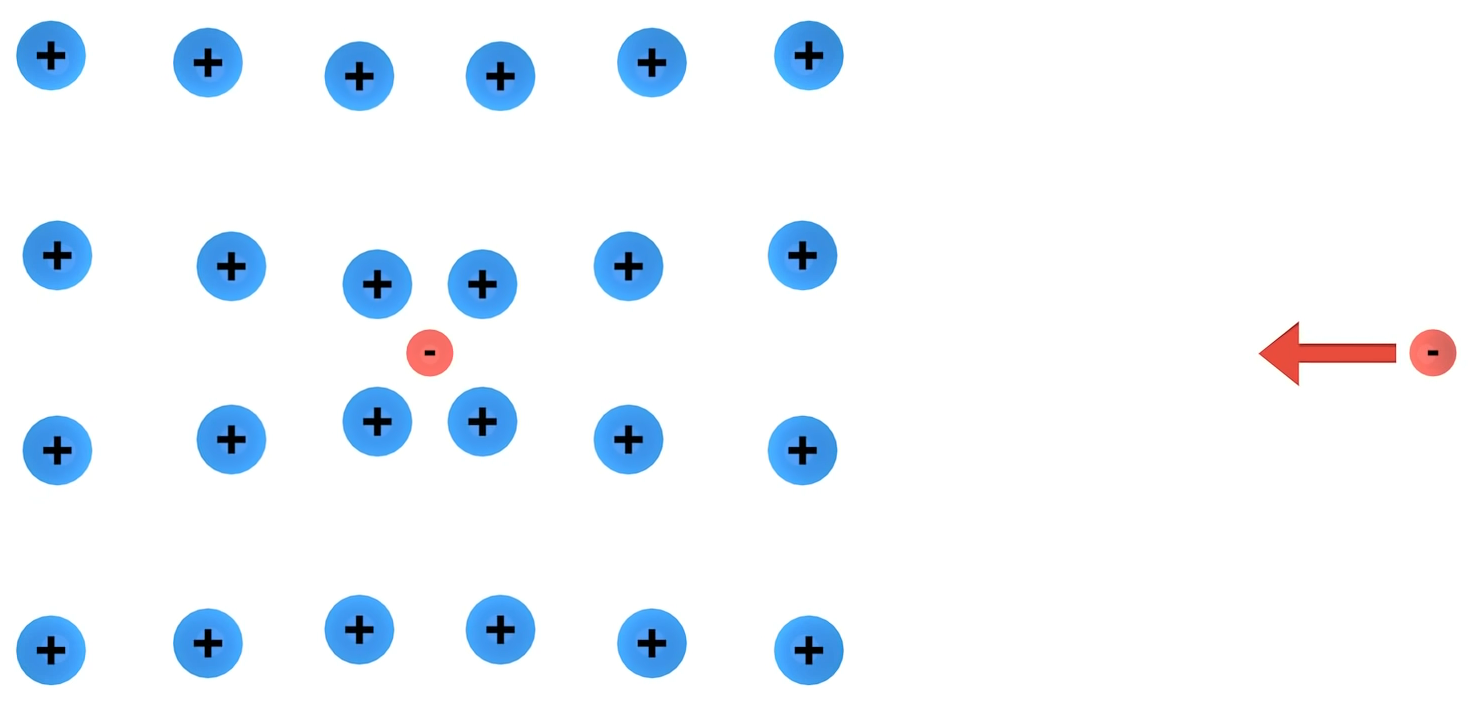
\includegraphics[width=0.6\linewidth]{fig/phonon.png}
\label{fig:phonon}
\caption{Ilustração da atração efetiva entre dois elétrons, mediada por fônons. Podemos interpretá-la classicamente como um elétron atraindo os íons positivos da rede para si, surgindo um acúmulo de carga positiva que leva um segundo elétron a sentir atração.}
\end{figure}

\n

\item Os pares de Cooper são bósons e condensam, formando um superfluido carregado.

\item Os estados de partícula única possuem dispersão $E_{\k} = \sqrt{\eps_{\k}^2 + \abs{\Delta}^2}$, onde o gap $\Delta$ não depende de $\k$ (esfericamente simétrico, ou s-wave).
\end{enumerate}

%%%%%%%%%%%%%%%%%%%%%%%%%%%%%%%%%%%%%%%%%%%%%%%%%%%%%%%%%%%%%%%%%%%%%%%%%%%%%%%%%%%%%%%%%%%%%%%%%


Visando generalizar as hipóteses acima, pensaremos num supercondutor não-convencional como ainda sendo formado pela criação de pares de Cooper, mas agora não assumimos que a atração atrativa é causada necessariamente por fônons e permitiremos uma função de gap $\Delta_{\k}$ dependente do momento. Dessa maneira, uma hamiltoniana que descreve pares de Cooper tem a forma geral
\begin{equation} \label{eq:hamilbcs}
H_I =
\frac{1}{V} \sum_{\k,\k'} V_{\k,\k'} (c_{\k\up}^\d c_{-\k\down}^\d) (c_{-\k'\down} c_{\k'\up}).
\end{equation}

Se definirmos $\Delta_{\k} = \sum_{\k'} V_{\k,\k'} \ev{c_{-\k'\down} c_{\k'\up}}$ e aplicarmos o procedimento de campo médio $AB \simeq A\ev{B} + B\ev{A} - \ev{A}\ev{B}$ para os operadores $A = \Psi_{\k}^\d = c_{\k\up}^\d c_{-\k\down}^\d$ e $B = \Psi_{\k'} = c_{-\k'\down} c_{\k'\up}$, generalizamos a \textit{equação do gap}
\begin{equation} \label{eq:gapeq}
\Delta_{\k} = - \frac{1}{V} \sum_{\k'} V_{\k,\k'} \frac{\Delta_{\k'}}{2 E_{\k'}} \tanh(\frac{\beta E_{\k'}}{2}).
\end{equation}

Devido ao sinal negativo acima, se $V_{\k,\k'}$ não for sempre negativo, a função de gap $\Delta_{\k}$ poderá ser negativa em alguns pontos, de maneira a surgirem nós ($\Delta_{\k} = 0$). A existência desses nós acontece em várias classes de supercondutores, como os orgânicos, heavy-fermion, cupratos e baseados em ferro.

%%%%%%%%%%%%%%%%%%%%%%%%%%%%%%%%%%%%%%%%%%%%%%%%%%%%%%%%%%%%%%%%%%%%%%%%%%%%%%%%%%%%%%%%%%%%%%%%%
\end{section}

\begin{section}{Termos de interação}

Tendo em mente o objetivo de capturar os nós da função de gap, faremos considerações gerais sobre duas classes de potenciais, de maneira a estudar como a anisotropia de $\Delta_{\k}$ pode surgir. Consideremos primeiramente um potencial repulsivo genérico
\begin{equation} \label{eq:repulsivo}
V = \frac{1}{2} \sum_{\substack{\k_1,\k_2,\q \\ \s, \s'}} V_{\q} c_{\k_1+\q,\s}^\d c_{\k_2+\q,\s'}^\d c_{\k_2,\s'} c_{\k_1,\s},
\end{equation}
e depois um ``magnético''
\begin{equation} \label{eq:magnetico}
V_{\text{mag}} = \sum_{i,j} J_{ij} \, \vb{S}_i \vdot \vb{S}_j = \frac{1}{2} \sum_{\q} J_{\q} \, \vb{S}_{-\q} \vdot \vb{S}_{\q}.
\end{equation}

\subsection{Potencial repulsivo}

Como estamos interessados na projeção nos pares de Cooper (momento total zero), consideramos que $\k_1 = -\k_2 = \k'$, $\k_1 + \q = -(\k_2 - \q) = \k$ e $\q = \k - \k'$. A interação resultante da equação \ref{eq:repulsivo} pode então ser separada nos spins
$$
V_{BCS} = \frac{1}{2} \sum_{\substack{\k,\k' \\ \s, \s'}} V_{\k-\k'} c_{\k\s}^\d c_{-\k\s'}^\d c_{-\k'\s'}c_{\k'\s} =
V_{BCS}^{\up\down} + V_{BCS}^{\up\up} + V_{BCS}^{\down\down}.
$$

Foquemos primeiramente no termo mais familiar (c.f. equação \ref{eq:hamilbcs})
\begin{equation} \label{eq:updown}
V_{BCS}^{\up\down} = \sum_{\k,\k'} V_{\k-\k'} (c_{\k\up}^\d c_{-\k\down}^\d) (c_{-\k'\down} c_{\k'\up}) =
\sum_{\k,\k'} V_{\k-\k'} \Psi_{\k}^\d \Psi_{\k'}.
\end{equation}

%%%%%%%%%%%%%%%%%%%%%%%%%%%%%%%%%%%%%%%%%%%%%%%%%%%%%%%%%%%%%%%%%%%%%%%%%%%%%%%%%%%%%%%%%%%%%%%%%

Olhemos os operadores de paridade $P$ e troca de spin $X$ da função de onda $F(\k)_{\alpha\beta} = \braket{\k\alpha,-\k\beta}{\k_P}$ do par de Cooper, definidos por
$$
P F(\k)_{\alpha\beta} = F(-\k)_{\alpha\beta},
$$
$$
X F(\k)_{\alpha\beta} = F(\k)_{\beta\alpha}.
$$

É imediato que o operador de troca de spin $X$ distingue estados de singleto $X = -1$ de tripleto $X = +1$ no espaço produto tensorial de momentos angulares $\frac{1}{2} \otimes \frac{1}{2} = 0 \oplus 1$. Lembremos que um par de spins $\ket{\up\down}$ não é singleto e nem tripleto. De fato, o singleto é $(\ket{\up\down} - \ket{\down\up})/\sqrt{2}$ e o tripleto é gerado pelos estados $(\ket{\up\down} + \ket{\down\up})/\sqrt{2}$, $\ket{\up\up}$ e $\ket{\down\down}$.

\n

Quando aplicamos $P$ e $X$ na função de onda $\braket{\k\alpha,-\k\beta}{\k_P}$ do par de Cooper, estaremos trocando os dois férmions que compõem o par. Essa operação composta deve adquirir uma fase $-1$ pela regra de anticomutação dos férmions. Portanto, temos que $PX = -1$ no subespaço dos pares de Cooper. Disso, imediamente concluimos que pares com paridade par $P = +1$ são singletos $(P,X) = (+, -)$ e com paridade ímpar $P = -1$ são tripletos $(P,X) = (-,+)$.

\n

Com os autovalores dos operadores $P$ e $X$ em mente, podemos decompor a interação \ref{eq:updown} em partes simétrica (paridade par, singleto) e antissimétrica (paridade ímpar, tripleto):
\begin{equation} \label{eq:singtrip}
V_{BCS}^{\up\down} = \sum_{\k,\k'}
\Bigg[
\overbrace{\qty(\frac{V_{\k-\k'} + V_{\k+\k'}}{2})}^{V_{\k,\k'}^S} +
\overbrace{\qty(\frac{V_{\k-\k'} - V_{\k+\k'}}{2})}^{V_{\k,\k'}^T}
\Bigg] \Psi_{\k}^\d \Psi_{\k}.
\end{equation}

O primeiro termo da equação \ref{eq:singtrip} espalha estado de singletos e o segundo de tripletos, que podem ser representados algebricamente por
$$
\Psi_{\k}^{S\d} = (c_{\k\up}^\d c_{-\k\down}^\d + c_{-\k\up}^\d c_{\k\down}^\d),
\quad \Psi_{\k}^{S\d} = +\Psi_{-\k}^{S\d},
$$
$$
\Psi_{\k}^{T\d} = (c_{\k\up}^\d c_{-\k\down}^\d - c_{-\k\up}^\d c_{\k\down}^\d),
\quad \Psi_{\k}^{T\d} = -\Psi_{-\k}^{T\d},
$$
de maneira a reescrever a interação \ref{eq:singtrip} na forma desacoplada
$$
V_{BCS}^{\up\down} =
\frac{1}{4} \sum_{\k,\k'}
\qty[
V_{\k,\k'}^S \Psi_{\k}^{S\d} \Psi_{\k'}^{S} +
V_{\k,\k'}^T \Psi_{\k}^{T\d} \Psi_{\k'}^{T}
].
$$

%%%%%%%%%%%%%%%%%%%%%%%%%%%%%%%%%%%%%%%%%%%%%%%%%%%%%%%%%%%%%%%%%%%%%%%%%%%%%%%%%%%%%%%%%%%%%%%%%

Os outros termos de spins paralelos $V_{BCS}^{\up\up}$ e $V_{BCS}^{\down\down}$ somente envolvem tripletos, que interagem via $V_{\k,\k'}^T$. Pulando alguns passos algébricos, se definirmos o vetor tripleto
$$
\va*{\Psi}_{\k}^T = \sum_{\alpha\beta} c_{\k\alpha}^\d \qty(\va*{\s} i \s_2)_{\alpha\beta} c_{-\k\beta}^\d =
\begin{cases}
\; \; \; \; c_{\k\down}^\d c_{-\k\down} - c_{\k\up}^\d c_{-\k\up}^\d \; , \quad (x) \\
\; i (c_{\k\down}^\d c_{-\k\down} + c_{\k\up}^\d c_{-\k\up}^\d), \quad (y) \\
\; \; \; \; c_{\k\up}^\d c_{-\k\down}^\d + c_{-\k\up}^\d c_{\k\down}^\d \; , \quad (z),
\end{cases}
$$
também conseguimos escrever as interações de spins paralelos de maneira desacoplada e compacta. No final obtemos
\begin{equation} \label{eq:desacoplado}
V_{BCS} =
V_{BCS}^{\up\down} + V_{BCS}^{\up\up} + V_{BCS}^{\down\down} =
\frac{1}{4} \sum_{\k,\k'}
\qty(
V_{\k,\k'}^S \Psi_{\k}^{S\d} \Psi_{\k'}^S +
V_{\k,\k'}^T \va*{\Psi}_{\k}^{T\d} \va*{\Psi}_{\k'}^T
).
\end{equation}

%%%%%%%%%%%%%%%%%%%%%%%%%%%%%%%%%%%%%%%%%%%%%%%%%%%%%%%%%%%%%%%%%%%%%%%%%%%%%%%%%%%%%%%%%%%%%%%%%

Tendo em mente os conceitos de paridade $P$, troca de spin $X$ e a forma desacoplada \ref{eq:desacoplado} do potencial, podemos colher algumas observações relevantes:


\begin{itemize}
\item Ao estudarmos os harmônicos esféricos $Y_{\ell m}$ no contexto do átomo de Hidrogênio, vemos que a paridade está associada ao número quântico de momento angular orbital $\ell$, de maneira que $Y_{\ell m}(-\r) = (-1)^\ell Y_{\ell m}(\r)$. Trazendo esse conhecimento para o contexto das funções de onda dos pares de Cooper, temos que os estados de singleto envolvem $\ell = 0, 2, \ldots$ (s, d, $\ldots$ wave) e que os de tripleto envolvem valores ímpares $\ell = 1, 3, \ldots$ (p, f, $\ldots$ wave).

\begin{figure}[H]
\centering
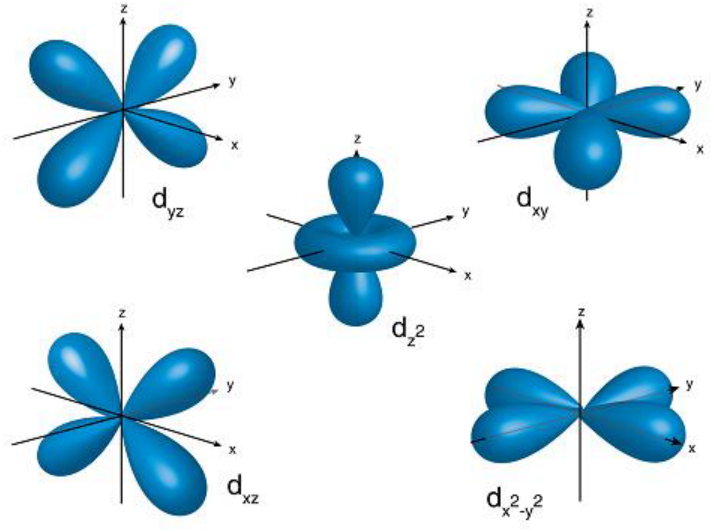
\includegraphics[width=0.55\linewidth]{fig/d-orbitals.png}
\caption{Harmônicos esféricos $Y_{2m}$ dos orbitais $d$.}
\label{fig:d-orbitals}
\end{figure}

\item Já que o potencial repulsivo $V_{BCS}$ se dissocia em interações de singleto e tripleto, podemos estudá-las separadamente. Em especial, só precisamos considerar o termo de tripleto $V^T_{\k,\k'}$ se estivermos interessados em descrever a simetria p-wave, por exemplo no estado superfluido do $^3$He.

\n

\item Para um acoplamento somente de singleto (caso das simetrias s-wave e d-wave), ficamos apenas com a hamiltoniana BCS da equação \ref{eq:hamilbcs}. Utilizaremos-a na seção \ref{sec:cupratos} para estudar a simetria d-wave dos cupratos.
\end{itemize}

\subsection{Potencial magnético}

Analisemos agora a interação magnética \ref{eq:magnetico}, que é do tipo Heisenberg
$$
V_{\text{mag}} = \frac{1}{2} \sum_{\q} J_{\q} \, \va*{S}_{-\q} \vdot \va*{S}_{\q} =
\frac{1}{2} \sum_{\substack{\k_1,\k_2,\q \\ \alpha\beta\gamma\delta}} J_{\q} c_{\k_1+\q,\alpha}^\d c_{\k_2-\q,\gamma}^\d
\qty(\frac{\va*{\s}}{2})_{\alpha\beta} \qty(\frac{\va*{\s}}{2})_{\gamma\delta} c_{\k_2\delta} c_{\k_1\beta},
$$
onde $J_{\q}$ é a interação efetiva dos spins. Por exemplo, para spins em uma rede quadrada interagindo só com primeiros vizinhos temos $J_{\q} = 2 J [\cos(q_x a) + \cos(q_y a)]$ (dispersão tight-binding).

\n

Considerando o produto escalar $\qty(\frac{\va*{\s}}{2})_{\alpha\beta} \cdot \qty(\frac{\va*{\s}}{2})_{\gamma\delta} \equiv \va*{S}_1 \vdot \va*{S}_2$, lembremos que seus autovalores são $+\frac{1}{4}$ para o tripleto e $-\frac{3}{4}$ para o singleto. Esse é um cálculo que geralmente é feito em cursos de Mecânica Quântica ao analisar a estrutura hiperfina do átomo de Hidrogênio.
\begin{equation} \label{eq:spineig}
\va*{S}_1 \vdot \va*{S}_2 =
\begin{cases}
\; +\frac{1}{4} \quad \text{(tripleto)}, \\
\; -\frac{3}{4} \quad \text{(singleto)}.
\end{cases}
\end{equation}

%%%%%%%%%%%%%%%%%%%%%%%%%%%%%%%%%%%%%%%%%%%%%%%%%%%%%%%%%%%%%%%%%%%%%%%%%%%%%%%%%%%%%%%%%%%%%%%%%


Já que as partes simétricas e antissimétricas da interação filtram os pares singleto e tripleto, temos que esses autovalores entram como prefatores no potencial, de maneira que
$$
V_{\k,\k'}^S = -\frac{3}{4} \qty(\frac{J_{\k-\k'} + J_{\k+\k'}}{2}), \quad
V_{\k,\k'}^T = +\frac{1}{4} \qty(\frac{J_{\k-\k'} - J_{\k+\k'}}{2}).
$$

Assim, ambas as interações antiferromagnéticas ($J > 0 \implies V_{\k,\k'}^S < 0$) e ferromagnéticas ($J < 0 \implies V_{\k,\k'}^T < 0$) causam uma interação efetiva atrativa nos pares de singleto e tripleto, respectivamente.

Podemos então explicitar as correspondências qualitativas:
$$
\begin{cases}
\; \text{interação antiferromagnética} \leftrightarrow \text{pares singleto anisotrópicos (e.g. d-wave),} \\
\; \text{interação ferromagnética} \leftrightarrow \text{pares tripleto anisotrópicos (e.g. p-wave).}
\end{cases}
$$

A saber, o estado normal (não-dopado) dos cupratos em geral é dado por um isolante de Mott com ordem antiferromagnética. Na próxima seção daremos foco especial a eles.

\end{section}

%%%%%%%%%%%%%%%%%%%%%%%%%%%%%%%%%%%%%%%%%%%%%%%%%%%%%%%%%%%%%%%%%%%%%%%%%%%%%%%%%%%%%%%%%%%%%%%%%


\begin{section}{Cupratos} \label{sec:cupratos}

Com o propósito de modelar fenomenologicamente a supercondutividade nos cupratos, primeiro listaremos fatos experimentais sobre essa classe de materiais.

\begin{minipage}{0.25\textwidth}
\begin{figure}[H]
\centering
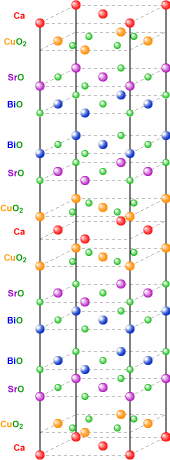
\includegraphics[width=\textwidth]{fig/bscco-unitcell.png}
\caption{Célula unitária do cuprato BSCCO-2212.}
\label{fig:bscco-unitcell}
\end{figure}
\end{minipage}
\begin{minipage}{0.65\textwidth}
  \begin{itemize}
  \item Os cupratos consistem de várias camadas de CuO$_2$, que possui uma rede quadrada. Na Figura \ref{fig:bscco-unitcell} ao lado vemos essas camadas na célula unitária do BSCCO-2212.
  \item O estado normal dos cupratos geralmente é um isolante de Mott com ordem antiferromagnética. Na Figura \ref{fig:cuprate-phasediag} essa fase antiferromagnética corresponde à região de cor laranja, em torno da região de dopagem nula.
  \item Quando superdopados os cupratos se comportam como líquidos de Fermi (metais). Essa fase metálica corresponde à região em azul no canto direito da Figura \ref{fig:cuprate-phasediag}.
  \item A interação atrativa elétron-elétron não é causada por fônons. Acredita-se que a atração seja devido à interação antiferromagnética, capaz de gerar supercondutividade d-wave.
  \end{itemize}
\end{minipage}


\begin{figure}[H]
\centering
\begin{subfigure}{.5\textwidth}
  \centering
  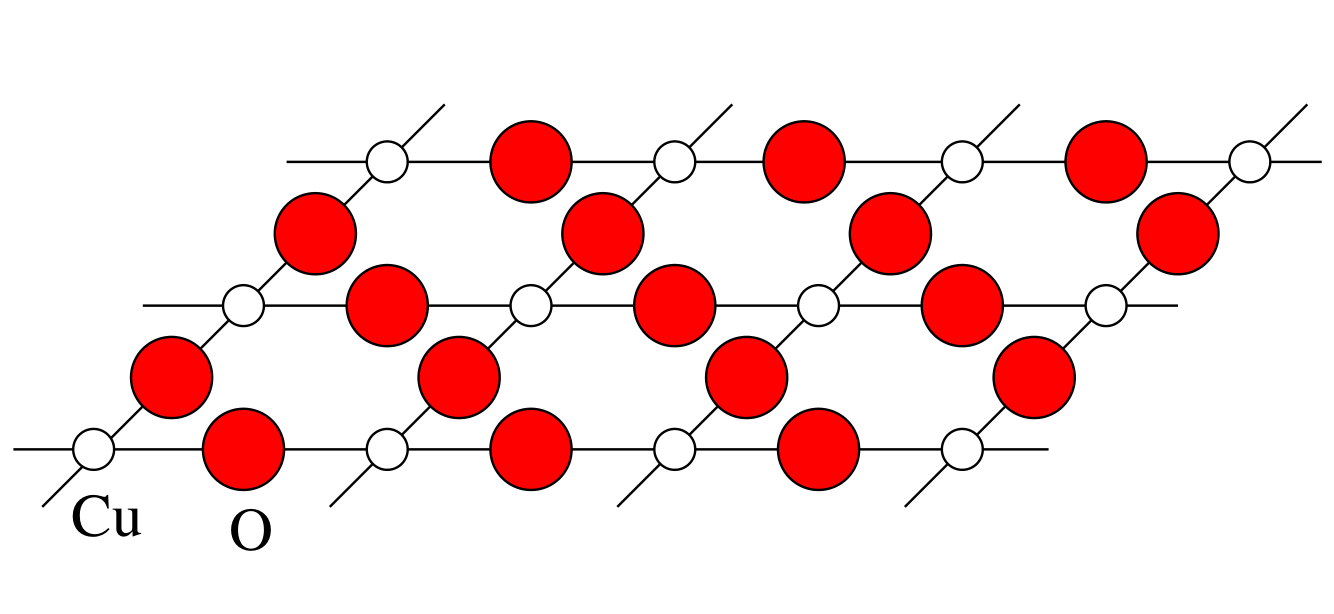
\includegraphics[width=\linewidth]{fig/cuo2.png}
  \caption{}
  \label{fig:cuo2}
\end{subfigure}
\begin{subfigure}{.34\textwidth}
  \centering
  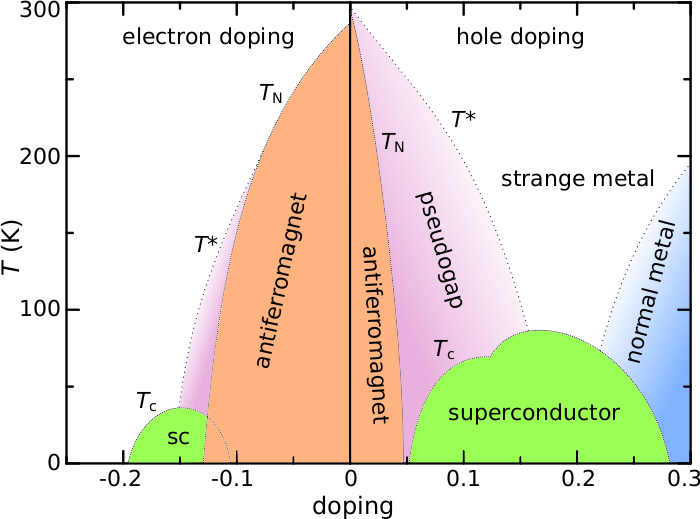
\includegraphics[width=\linewidth]{fig/cuprate-phasediag.png}
  \caption{}
  \label{fig:cuprate-phasediag}
\end{subfigure}
\caption{(a) Os cupratos possuem planos de CuO$_2$, que forma rede quadrada. (b) Diagrama de fase de dopagem por temperatura representativo dos cupratos.}
\label{fig:cuprates}
\end{figure}

A abordagem discutida na seção \ref{sec:bcs} assume que o estado normal do material é um líquido de Fermi. Olhando para o diagrama de fase da Figura \ref{fig:cuprate-phasediag} vemos que isso não é verdade para os cupratos à dopagem nula, mas sim quando eles estão superdopados (dopagem $\simeq 0.3$). Mesmo assim, esperamos que a fenomenologia BCS nos possibilite explorar a simetria d-wave do estado supercondutor dos cupratos.

\n

Tendo em vista as propriedades discutidas dos cupratos, consideramos um modelo simplificado de um supercondutor d-wave para os cupratos, onde os elétrons se movem em uma rede quadrada com dispersão $\eps_{\k} = -2t (\cos k_x a + \cos k_y a)$. Incluimos a repulsão de Coulomb por meio de um termo local de Hubbard e também consideramos interações antiferromagnéticas para primeiros vizinhos:
$$
H = \sum_{\k} \eps_{\k} c_{\k\s}^\d c_{\k\s} + \sum_{j} U n_{j\up} n_{j\down} + J \sum_{\nn{i}{j}} \va*{S}_i \vdot \va*{S}_j.
$$

Supondo que $U, J \ll t$, tratamos o material como um líquido de Fermi com uma interação BCS de singleto
$$
V^{\text{singleto}}(\q) = U - \frac{3J}{2} (\cos q_x a + \cos q_y a),
$$
onde o fator $-\frac{3}{2}$ surge do autovalor de singleto $-\frac{3}{4}$ da equação \ref{eq:spineig}.

\n

A interação $V_{\k,\k'}$ é obtida a partir da simetrização
$$
V_{\k,\k'} = \frac{1}{2}
\Big[
V^{\text{singleto}}(\k-\k') + V^{\text{singleto}}(\k+\k')
\Big] =
U - \frac{3}{2} (c_x c_{x'} + c_y c_{y'}),
$$
onde denotamos $c_x = \cos(k_x a)$ e $c_y = \cos(k_y a)$. A hamiltoniana BCS é então
$$
H_{BCS} = \sum_{\k\s} \eps_{\k} c_{\k\s}^\d c_{\k\s} +
\sum_{\k,\k'} \qty[U - \frac{3}{2} (c_x c_{x'} + c_y c_{y'})]
c_{\k\up}^\d c_{-\k\down}^\d c_{-\k'\down} c_{\k'\up}.
$$


Podemos separar a interação $V_{\k,\k'} = V_{\k,\k'}^s + V_{\k,\k'}^d$ em um termo s-wave e d-wave:
$$
V_{\k,\k'}^s =
\overbrace{U}^{\text{s-wave}} -
\overbrace{\frac{3}{4} J (c_x + c_y) (c_{x'} + c_{y'})}^{\text{s-wave estendida}}
\quad \text{(s-wave)},
$$
$$
V_{\k,\k'}^d = - \frac{3}{4} J (c_x - c_y) (c_{x'} - c_{y'})
\quad \text{(d-wave)},
$$
onde o termo s-wave é invariante por rotações de $90^\circ$ e o termo d-wave troca de sinal, $V_{\k,\k'}^s = + V_{\k, R\k'}^s$ e $V_{\k,\k'}^d = - V_{\k, R\k'}^d$ com $R\k = (-k_y, k_x)$.

\n

Se analisarmos a equação \ref{eq:gapeq} do gap
$$
\Delta_{\k} = - \int \frac{\dd[2]{\k'}}{(2\pi)^2} (V_{\k,\k'}^s + V_{\k,\k'}^d) \frac{\Delta_{\k'}}{2 E_{\k'}} \tanh(\frac{\beta E_{\k'}}{2}),
$$
é possível escrever também $\Delta_{\k} = \Delta_{\k}^s + \Delta_{\k}^d$, com
$$
\Delta_{\k}^s = \Delta_1 + \Delta_ 2 (c_x + c_y) = + \Delta_{R\k}^s,
$$
$$
\Delta_{\k}^d = \Delta_d (c_x - c_y) = - \Delta_{R\k}^d.
$$

Os dois termos $\Delta_{\k}^s$ e $\Delta_{\k}^d$ se acoplam somente com as respectivas interações s-wave e d-wave na equação do gap, pois $\int \frac{\dd[2]{\k'}}{(2\pi)^2} V_{\k,\k'}^s \Delta^d_{\k'} (\ldots) = 0$ e $\int \frac{\dd[2]{\k'}}{(2\pi)^2} V_{\k,\k'}^d \Delta^s_{\k'} (\ldots) = 0$, devido às integrais mudarem de sinal sob uma rotação de $90^\circ$ e, portanto, serem nulas. Concluimos que as duas simetrias s-wave e d-wave são desacopladas e que, em particular, a simetria d-wave é ortogonal ao potencial de Coulomb local $U$.


\n


Analisando o gap d-wave $\Delta_{\k}^d = \Delta_d (c_x - c_y)$, vemos que ele possui nós nas diagonais $k_x = \pm k_y$, de maneira que essa simetria d-wave tem a forma do orbital $d_{x^2-y^2}$ da Figura \ref{fig:d-orbitals}. A energia das quasepartículas $E_{\k} = \sqrt{\eps_{\k}^2 + \Delta_d^2 (c_x - c_y)^2}$ se anula na interseção dessas diagonais (onde $\Delta_{\k} = 0$) com a superfície de Fermi (onde $\eps_{\k} = 0$), de maneira a formar cones de Dirac nesses pontos (nodais), ilustrados na Figura \ref{fig:fermisurf}.

\begin{figure}[H]
\centering
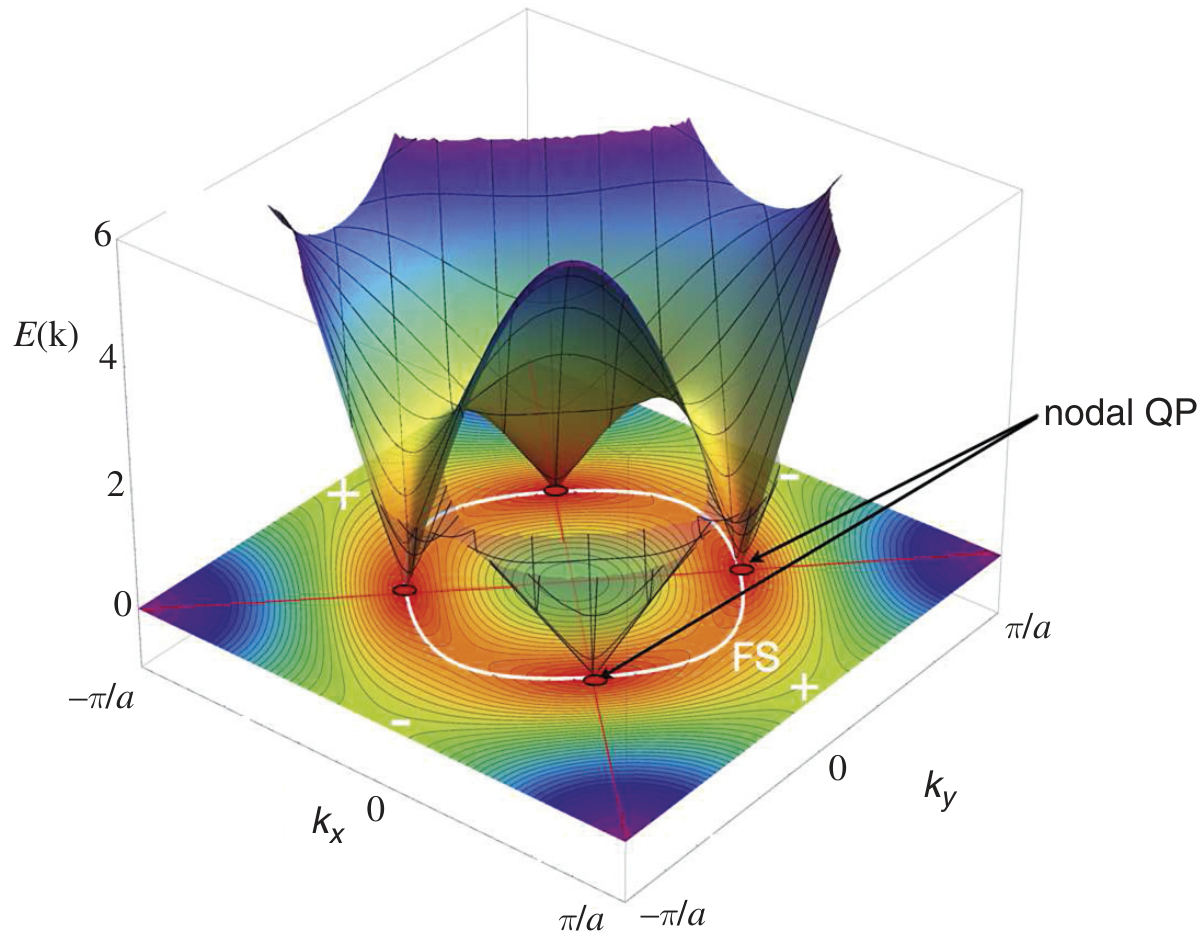
\includegraphics[width=0.8\linewidth]{fig/fermisurf.png}
\caption{Cones de Dirac nos pontos nodais, que se localizam na interseção da superfície de Fermi (FS) com as retas $k_x = \pm k_y$.}
\label{fig:fermisurf}
\end{figure}


Utilizando a equação do gap, podemos fazer algumas aproximações para ter uma ideia da física envolvida. Supondo que o preenchimento ao redor de $\Gamma (\k = \0)$ seja pequeno, temos $\eps_{\k} = -2t (c_x + c_y) \simeq -4t  + t k^2$ e o gap
$$
\Delta_{\k}^d = \Delta_d (c_x - c_y) \simeq -\frac{\Delta_d}{2 k_F^2}
\qty[\qty(\frac{k_x}{k_F})^2 - \qty(\frac{k_y}{k_F})^2] = - \Delta_0 \cos(2\theta),
\quad \Delta_0 = \frac{\Delta_d}{2 k_F^2}, \k = (k_x, k_y) = \abs{\k} e^{i\theta}.
$$

Em particular, observamos que $\Delta^d(\theta) \propto \cos(2\theta)$ remete ao harmônico esférico do orbital $d_{x^2 - y^2}$ da Figura \ref{fig:d-orbitals}.

\n

Colocando um cutoff na energia $\abs{\eps} \leq \omega_0$ e assumindo que a densidade de estados por spin seja constante $\rho(E_F) = \frac{1}{4\pi t}$, obtemos a equação do gap:
$$
1 = \frac{3 J}{4} \rho(E_F) \int_{-\omega_0}^{\omega_0} \dd{\eps}
\int_0^{2\pi} \frac{\dd{\theta}}{2\pi} \cos[2](2\theta) \frac{\tanh(\frac{\beta E}{2})}{2E}, \quad E = \sqrt{\eps^2 + [\Delta_0 \cos(2\theta)]^2}.
$$

Aproximando $\cos[2](2\theta)$ pela sua média $1/2$, chegamos numa equação do tipo BCS para $T_c$:
$$
1 = \frac{3J}{8} \rho(E_F) \int_0^{\omega_0} \dd{\eps} \,
\frac{\tanh(\frac{\eps}{2T_c})}{\eps},
$$
onde é possível obter $T_c \sim 1.13 \, \omega_0 e^{-\frac{8}{3 J \rho(E_F)}}$.


\n

Também podemos calcular a densidade de estados aproximada tomando uma média sobre o ângulo $\theta$:
$$
\frac{N_d(E)}{N(0)} = \dv{\eps}{E} =
\Re{\int_0^{2\pi} \frac{\dd{\theta}}{2\pi}
\frac{\abs{E}}{\sqrt{(E - i\delta)^2 + [\Delta_0 \cos(2\theta)]^2}}
},
$$
em que obtém-se a Figura \ref{fig:dwavedos}.

\begin{figure}[H]
\centering
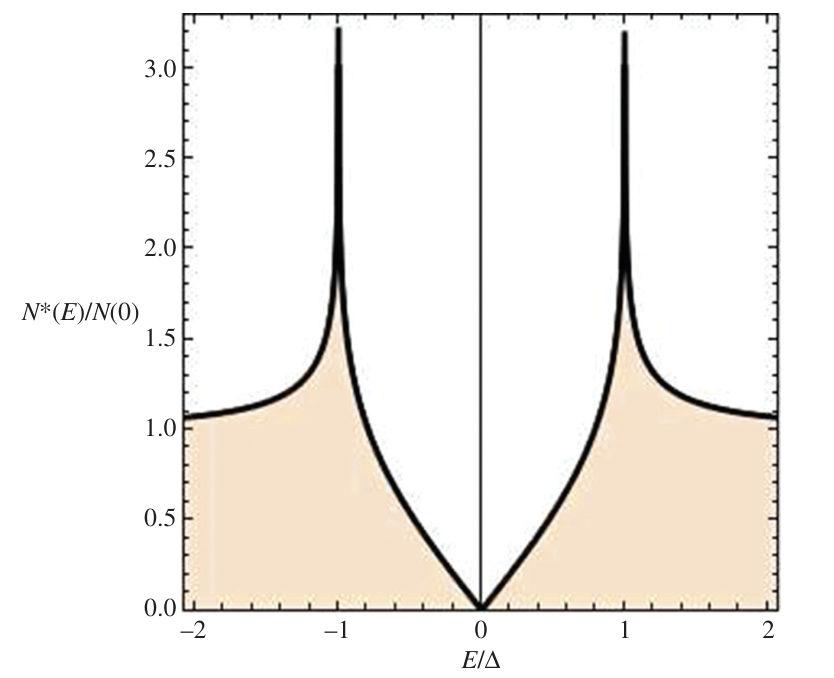
\includegraphics[width=0.6\textwidth]{fig/dwavedos.png}
\caption{Densidade de estados $N_d(E)/N(0)$ aproximada para um supercondutor d-wave.}
\label{fig:dwavedos}
\end{figure}

Note que não temos mais uma densidade de estados gapeada, pois de fato há cones de Dirac nos pontos nodais das diagonais $k_x = \pm k_y$. A Figura \ref{fig:dwavedos} na realidade se assemelha muito à densidade de estados do grafeno.

\n

Por final, exploremos a componente s-wave do gap $\Delta_{\k}^s = \Delta_1 + \Delta_2 (c_x + c_y)$. A equação do gap correspondente é
$$
\Delta_{\k}^s = - \int \frac{\dd[2]{\k'}}{(2\pi)^2}
\overbrace{\qty[U - \frac{3}{4} J (c_x + c_y)(c_{x'}+ c_{y'})]}^{V_{\k,\k'}^s}
\frac{\Delta_{\k'}^s}{2 E_{\k'}} \, \tanh(\frac{\beta E_{\k'}}{2}).
$$

Ela é mais complicada pois existe acoplamento entre o termo local $\Delta_1$ e o termo s-wave estendido $\Delta_2 (c_x + c_y)$.

\n

De forma simplificada, assumindo uma única superfície de Fermi, um cutoff $\abs{\eps} \leq \omega_0$ e expandindo $\k, \k' \ll t$ próximo do ponto $\Gamma$ de maneira que $c_x \simeq c_y \simeq 1$, temos que a interação efetiva é da ordem de $V_{\k,\k'}^s \simeq U - 3J$. Isso indica que, para uma única superfície de Fermi, a atração s-wave estendida é suprimida pela interação de Coulomb $U$. Isso faz com que a interação efetiva seja reduzida.

Pensando na fórmula da temperatura crítica BCS para a componente s-wave $T_c^s \sim 1.13 \, \omega_0 e^{-\frac{1}{g \rho(E_F)}}$, essa redução na constante efetiva de acoplamento $g \sim V_{\k,\k'}^s \simeq U-3J$ faz com que a temperatura crítica s-wave diminua. Essas estimativas indicam que nos cupratos o $T_c^d$ da componente d-wave é maior que $T_c^s$ (que foi suprimido por $U$), fazendo com que o pareamento d-wave seja predominante.

\end{section}


%%-----
%% Referências bibliográficas
%%-----
\addcontentsline{toc}{chapter}{\bibname}
%\bibliographystyle{abntex2-num}
\bibliography{citations}
\bibliographystyle{ieeetr}



\end{document}
